\documentclass[12pt]{extarticle}
\usepackage{tikz}
\usepackage{amsmath,amssymb}
\usepackage{caption}
\usepackage{graphicx}
\usepackage{multicol}
\usepackage{hyperref}
\usepackage{geometry}
\usepackage{watermark}
\usepackage{varwidth}
\usepackage{float}
\usepackage{arydshln}
\usepackage[dvipsnames]{xcolor}
\usepackage{tcolorbox}
\usepackage{booktabs}
%\usepackage{scrlayer-scrpage}
\usepackage{forest}
\usepackage{fancyhdr}
\pagecolor{white}
\geometry{bottom= 30mm}
\usepackage{enumitem}


\newcommand{\assignnumber}{\color{red}number\color{black}} %tell latex number of Homework

\title{Data Management Assignment 5}
\author{Cuihuan Zhang} 
\fancyhead[L]{Data Management}
\fancyhead[C]{Assignment 5}
\fancyhead[R]{Cuihuan Zhang}
\renewcommand\headrulewidth{0pt}
\pagestyle{fancy}
\pagenumbering{arabic}

\begin{document}

\maketitle \vspace{-10mm}
\rule{\linewidth}{0.4pt}


\begin{flushleft}
\begin{enumerate}

\item

\begin{enumerate}

\item

\begin{enumerate}
\item Scenarios when insertion from a heap would take 1 operation when the new record is directly insert in front (such like the head of a linked list) or null value of the block, without access the other data.
\item Scenarios when insertion from a heap would take N operations when the heap is compaction or cannot easily access the back of the heap. For example, insert the value in between, then we need to move the rest of the data.
\end{enumerate}

\item Scenarios when insertion from a sorted sequence would take log N + N operations: a sorted sequence requires log N using binary search to find the position, then move the rest of the data cost N when the sequence is compaction.

\item Scenarios when insertion from a 2-3 tree would take log N operations when insertion a integer without insert a new node. Just find the position (node) and insert the value when the node has null value of the block.
\end{enumerate}

\item
\begin{enumerate}

\item
\begin{enumerate}
\item 
A dense index contains a dedicated pointer (index entry) for every unique key value in the data file (number of indexes = number of records).
A sparse index contains pointers only for selected key values (e.g., the first key of each data block) (number of indexes < number of records). \\
For example: \\
Block1: [ID=1, Alice] → [ID=2, Bob] \\
Block2: [ID=3, Mary] → [ID=4, David] \\
Dense index file: \\
1 → Block1-Offset0 (Alice)  \\
2 → Block1-Offset1 (Bob)  \\
3 → Block2-Offset0 (Mary)  \\
4 → Block2-Offset1 (David)  \\
Sparse index file: \\
1 → Block1  \\
3 → Block2  \\

\item Sparse index requires less storage of the index file, which also leads to less index maintenance operations (no need for index maintenance operations when every time we need to insert or delete a value).
\end{enumerate}

\item A clustered index ensures that the physical order of records in the data file matches the logical order of the index keys.
An unclustered index is independent of the physical order of data records. \\
For example: \\
\begin{figure}[h]
  \centering
  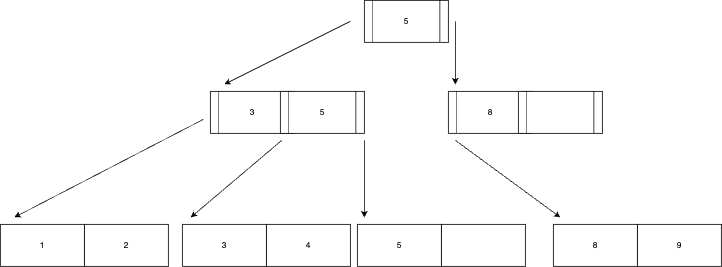
\includegraphics[width=0.8\textwidth]{clustered.drawio.png}
  \caption{clustered index}
\end{figure}

\begin{figure}[h]
  \centering
  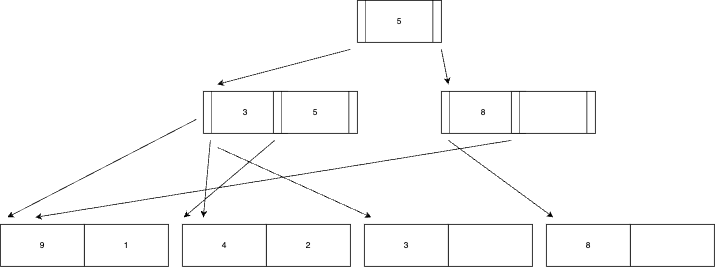
\includegraphics[width=0.8\textwidth]{unclustered.drawio.png}
  \caption{unclustered index}
\end{figure}

\item Best: sparse index and clustered file. High storage efficiency since only record the head of blocks. Less index maintenance operation since when inserting/deleting data, the update frequency of sparse indexes is lower than the dense indexes. High query speed since after locates the block by sparse index, the target record must be in the block.\\
Worest: sparse Index and unclustered file. Low query efficiency since after locates the centain block by sparse index, the target record may not include in the block due to the unclustered file. Require more storage since the localization of sparse indexes fails under the unclustered file, and additional redundant index entries may required to cover the scattered data. For example, require an additional dense and clustered index.

\end{enumerate}

\item

\begin{enumerate}
\item
\begin{itemize}
    \item \textbf{Disk size}: 5 GiB = \(5 \times 2^{30}\) bytes
    \item \textbf{Block size}: 256 bytes
    \item \textbf{Key size}: 8 bytes
    \item \textbf{Pointer size}: ?
\end{itemize}

\subsection*{Step-by-Step Calculation}

\paragraph{1. Total Number of Blocks:}
\[
\text{Number of blocks} = \frac{\text{Disk size}}{\text{Block size}} = \frac{5 \times 2^{30}}{256} = 5 \times 2^{22} = 20,\!971,\!520 \text{ blocks}
\]

\paragraph{2. Block Address Size:}
\[
\log_2(20,\!971,\!520) \approx 24.32 \text{ bits}
\]
\begin{itemize}
    \item Round up to 25 bits (requires \textbf{4 bytes} (\(4 \times 8\) = 32 bits, 1 byte = 8 bits) for alignment)
\end{itemize}

\paragraph{3. The largest possible number of children:}
Each node contains \(m\) pointers and \(m-1\) keys:
\[
m \times (\text{Pointer size}) + (m-1) \times (\text{Key size}) \leq \text{Block size}
\]
Substitute values (4 bytes pointers, 8 bytes keys):
\[
4m + 8(m-1) \leq 256
\]
\[
12m \leq 264 \implies m \leq 22
\]
\[
\boxed{m = 22}
\]
The smallest number of children are 11, and the largest number of children are 22.

\item

\begin{tabular}{cll}
\toprule
\textbf{Level} & \textbf{Nodes in a narrow tree (\(m=11\))} & \textbf{Nodes in a wide tree (\(m=22\))} \\
\midrule
1     & 1          & 1          \\
2     & 2          & 22         \\
3     & 22         & 484        \\
4     & 242        & 10,648     \\
5     & 2,662      & 234,256    \\
6     & 29,282     & --\\
7     & 322,102    & --\\
8     & 3,543,122  & --\\
\bottomrule
\end{tabular}

\item I will use B+ trees because the quantity involves range queries. Quickly locate all records within the interval through the traversal of the B+ tree structure.

\end{enumerate}

\item Order of joins
\begin{itemize}
    \item Table \( R \): 2000 blocks.
    \item Table \( S \): 4000 blocks.
    \item Available RAM: 6 blocks (2 for \( R \), 4 for \( S \)).
\end{itemize}

\begin{enumerate}

\item Partitioning for S
\begin{align*}
    \text {Each chunk of S uses 4 blocks.} \\
    \text{Total outer chunks: } \frac{4000}{4} = 1000. \\
\end{align*}


\item Scanning S for Each Chunk of R
\begin{align*}
    \text {For each outer chunk (1000 total) and scan the entire R (2000 blocks).} \\
    \text{Total cost for R: } 1000 \times 2000 = 2,000,000 \text{ blocks.} \\
\end{align*}

\item Total Cost
\[
\text{Total Block Accesses} = 4,000 \,(S) + 2,000,000 \, (R) = \boxed{2,004,000}
\]
\end{enumerate}

\end{enumerate}
\end{flushleft}
\end {document}